%!TEX root = ../thesis.tex
%*******************************************************************************
%****************************** Second Chapter *********************************
%*******************************************************************************

\chapter{Experimental} % 1200 words as of sept 22

\ifpdf
    \graphicspath{{Chapter2/Figs/Raster/}{Chapter2/Figs/PDF/}{Chapter2/Figs/}}
\else
    \graphicspath{{Chapter2/Figs/Vector/}{Chapter2/Figs/}}
\fi


\section[Preparation of samples]{Preparation of pigment samples} 
\label{section2.1}

Reference samples were acquired from Dr. Spike Bucklow from the Hamilton Kerr Institute collection and Dr. Andrea Kirkham from her sample library. All were loose powder and are described qualitatively in Table \ref{table:ref_sample}. The sample descriptions provided formed the basis for interpretation of results (and some terminology such as "bice" is used to describe both natural and synthetic pigments---this ambiguity is discussed when analysing results). Samples are pictured in \textit{Figures \ref{fig:sample_bags}} and \textit{\ref{fig:sample_vials}}, and prepared for confocal Raman analysis in \textit{Figure \ref{fig:sample_slides}}.

Prior to Raman analysis, small quantities of each pigment were pressed onto double-sided sellotape and smoothed. Prior to SEM-EDS analysis, small quantities of each pigment were pressed onto high purity carbon tabs.

\begin{table}[H]
\caption{Reference sample descriptions}
\centering
\label{table:ref_sample}
\begin{tabular}{c c}
\toprule
Reference sample & Qualitative physical description \\
\midrule
HKI natural azurite & Natural azurite, medium sandy blue \\
HKI cross section & Natural and artifical azurite \\
KE1a, KE1b & Green bice, light pale teal green \\
KE2 & Green verditer, CuCO\textsubscript{3} $\cdot$ Cu(OH)\textsubscript{2}, bright teal green \\
KE3 & Light verditer bice, medium dark blue \\
KE4 & Blue bice, medium grey blue \\
KE5 & Blue verditer, 2CuCO\textsubscript{3} $\cdot$ Cu(OH)\textsubscript{2}, dark blue \\
Fitz1 & Blue verditer, Fitzpatrick 10180, dark blue \\
Az1 & Azurite, medium light blue \\
Az2 & Azurite, dark deep blue \\
AzOp & Azurite, medium blue \\
AzMag & Azurite, medium teal blue \\
Ma1 & Malachite, medium light green \\
\bottomrule
\end{tabular}
\end{table}

\begin{figure}[H]
\centering
  \includegraphics[width=0.75\linewidth]{sample_bags}
\caption[Samples KE1-5 and Fitz1.]{Samples KE1-5 and Fitz1 shown in storage bags.}
\label{fig:sample_bags}
\end{figure}

\begin{figure}[H]
\centering
  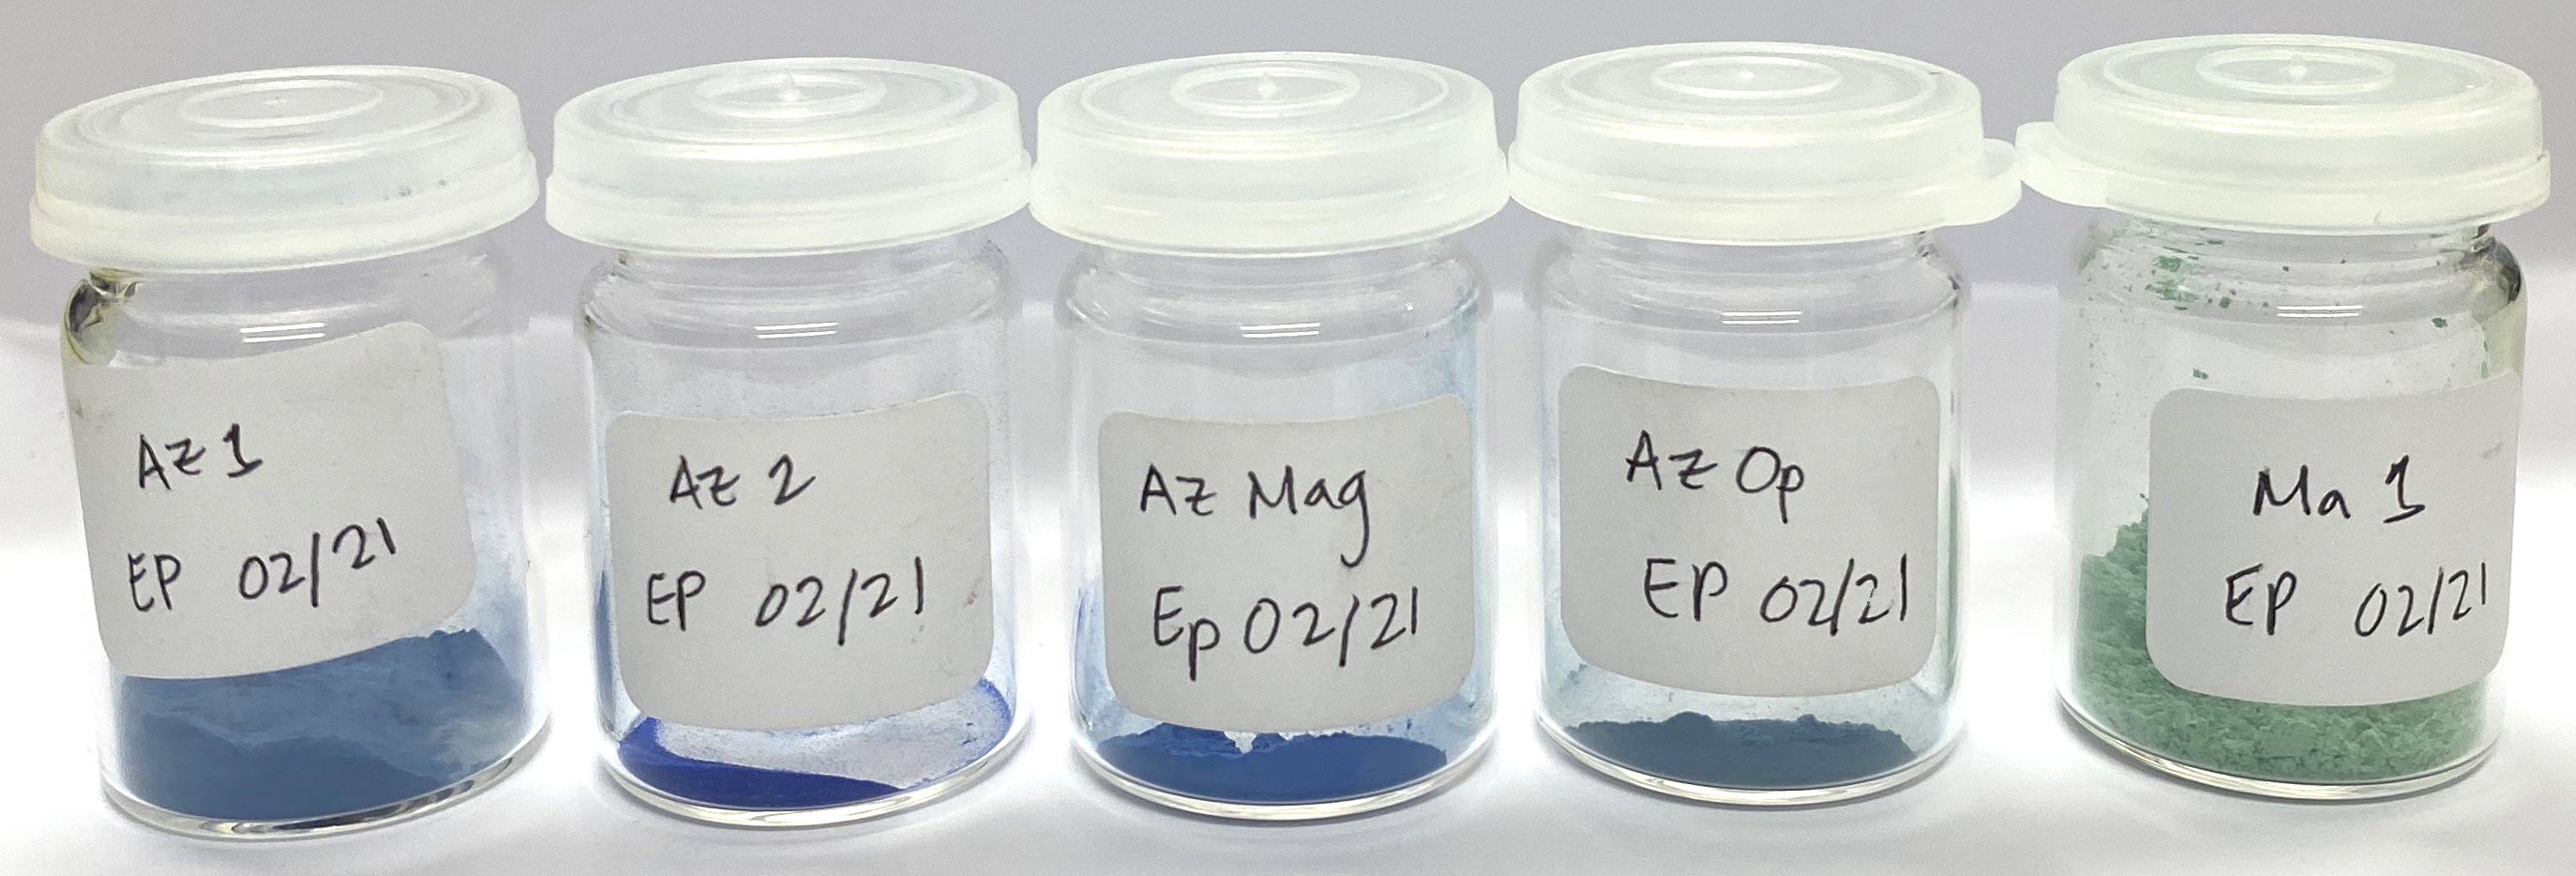
\includegraphics[width=0.75\linewidth]{sample_vials}
\caption[Samples Az1, Az2, AzOp, AzMag, and Ma1.]{Samples Az1, Az2, AzOp, AzMag, and Ma1, shown in small sample vials.}
\label{fig:sample_vials}
\end{figure}

\begin{figure}[H]
\centering
  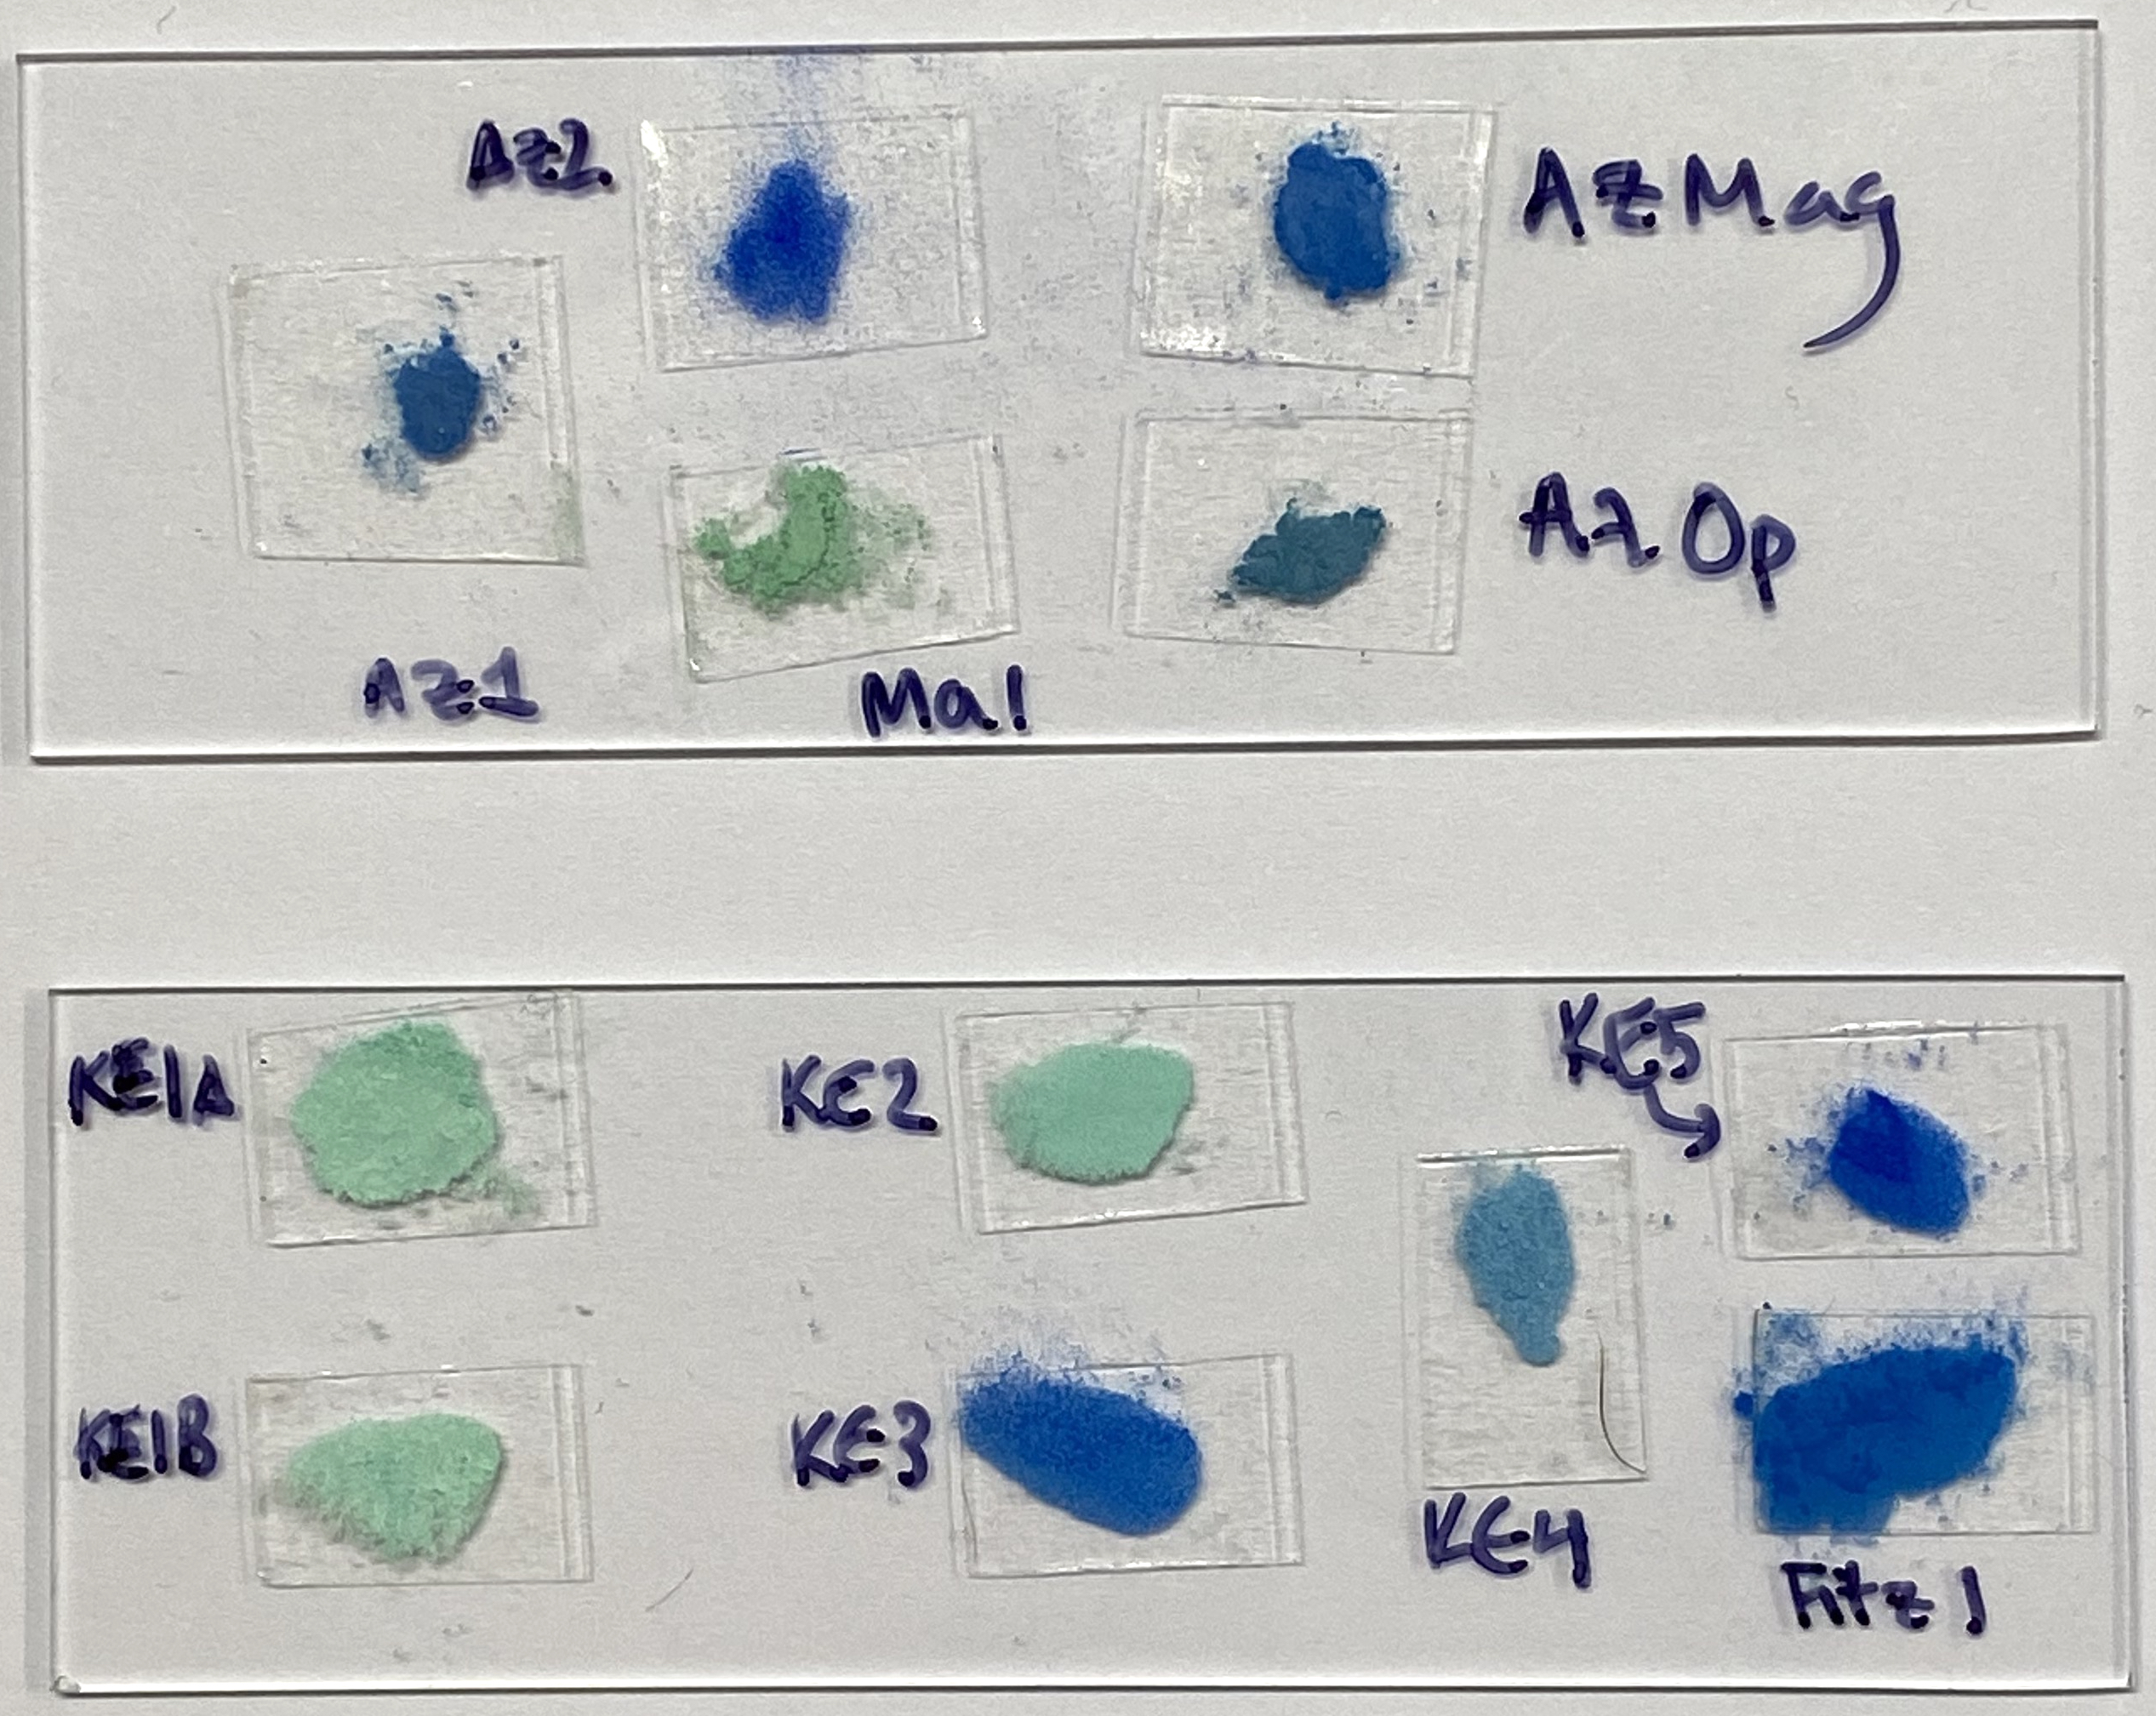
\includegraphics[width=0.75\linewidth]{sample_slides}
\caption[All reference samples shown pressed on double-sided tape and prepared for Raman analysis.]{All reference samples shown pressed on double-sided tape and prepared for Raman analysis.}
\label{fig:sample_slides}
\end{figure}

Samples were also embedded in polyester resin ((Tiranti clear casting resin) and polished for Raman mapping and AFM analysis. Samples were filed to approximately 5 mm in height and the pigment containing surface was polished using three sequential grit sizes of silicon carbide paper (English Abrasives) and polishing cloth (Buehler), using a fine grade cerium oxide polishing powder (Beckman-RIIC) in ethanol. Finally, samples were cleaned with ethanol.

\section[Analysis of pigment particles by Raman spectroscopy]{Analysis of pigment particles by Raman spectroscopy}
\label{section2.2}

Collection of Raman spectra was done using a Horiba LabRAM HR Evolution confocal Raman spectrometer, a 50x microscope objective (Olympus LMPLFLN), a 600 grooves/mm grating, 100 $\mu$m pinhole, and a CCD array (1024x1024 pixels). An laser with excitation wavelength of 532 nm (diode-pumped solid-state, Laser Quantum) was initially selected based on optimal signal and lack of sample damage. Azurite and malachite should show strong signals at 532 nm based on previous work.~\autocite{Bicchieri} References were also collected at 473 nm (Cobolt, 1800 grooves/mm grating, 150 $\mu$m pinhole), which showed superior results for blue samples due to high reflection but did not perform well on green samples. Two other excitation wavelengths, 633 nm and 785 nm, were also tested and found to be inferior (\textit{Figure \ref{fig:Az1_wavelength_comparison}}). Spectra were collected by focusing on specific pigment grains.

Resin-embedded cross section samples from \textit{Battle of Spurs} were studied using the same procedure.

\begin{figure}[H]
\centering
  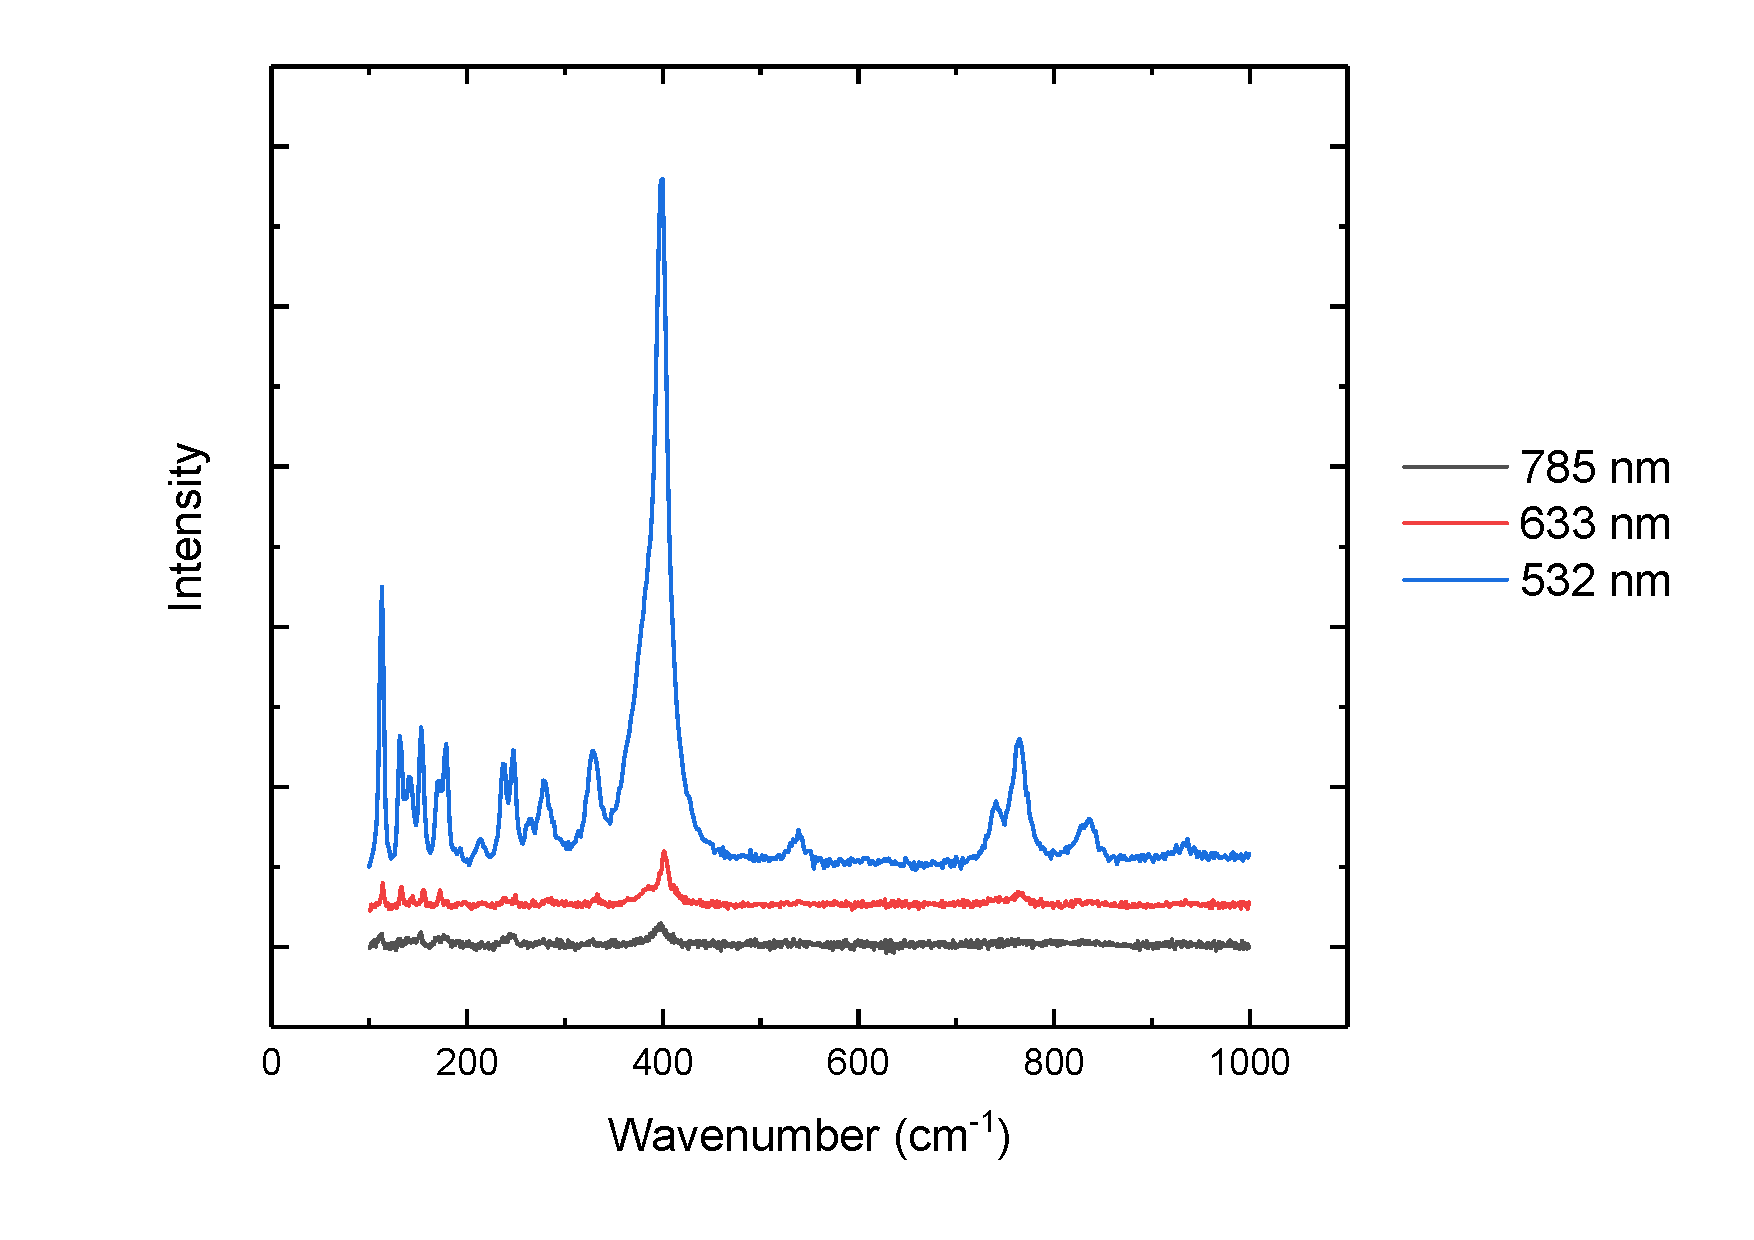
\includegraphics[width=0.75\linewidth]{Az1_wavelength_comparison}
\caption[Comparison of spectra collected at 473, 532, 633, and 785 nm excitation wavelengths from sample Az1.]{Comparison of spectra collected at 473 (green), 532 (blue), 633 (red), and 785 nm (black) excitation wavelengths from sample Az1.}
\label{fig:Az1_wavelength_comparison}
\end{figure}

Optimal collection parameters maximised the signal to noise ratio of spectra and avoided damage (\textit{Figure \ref{fig:Az1_laserpower_comp_532}}). The damage threshold of pigment grains depended on the sample and the grain size, also observed in previous studies.~\autocite{Cardell,Mattei} Damage to azurite (blue bice, blue verditer) samples occurred at 4 mW (10 s acquisition, 10 accumulations). Malachite (green verditer) has a lower damage threshold, 2 mW (10 s acquisition, 10 accumulations). 1 mW power with an acquisition time of 10 s and 10 accumulations did not cause observable damage to any sample and gave useable signal quality. To be consistent, this lower surface power and acquisition time was used. 

\begin{figure}[H]
\centering
  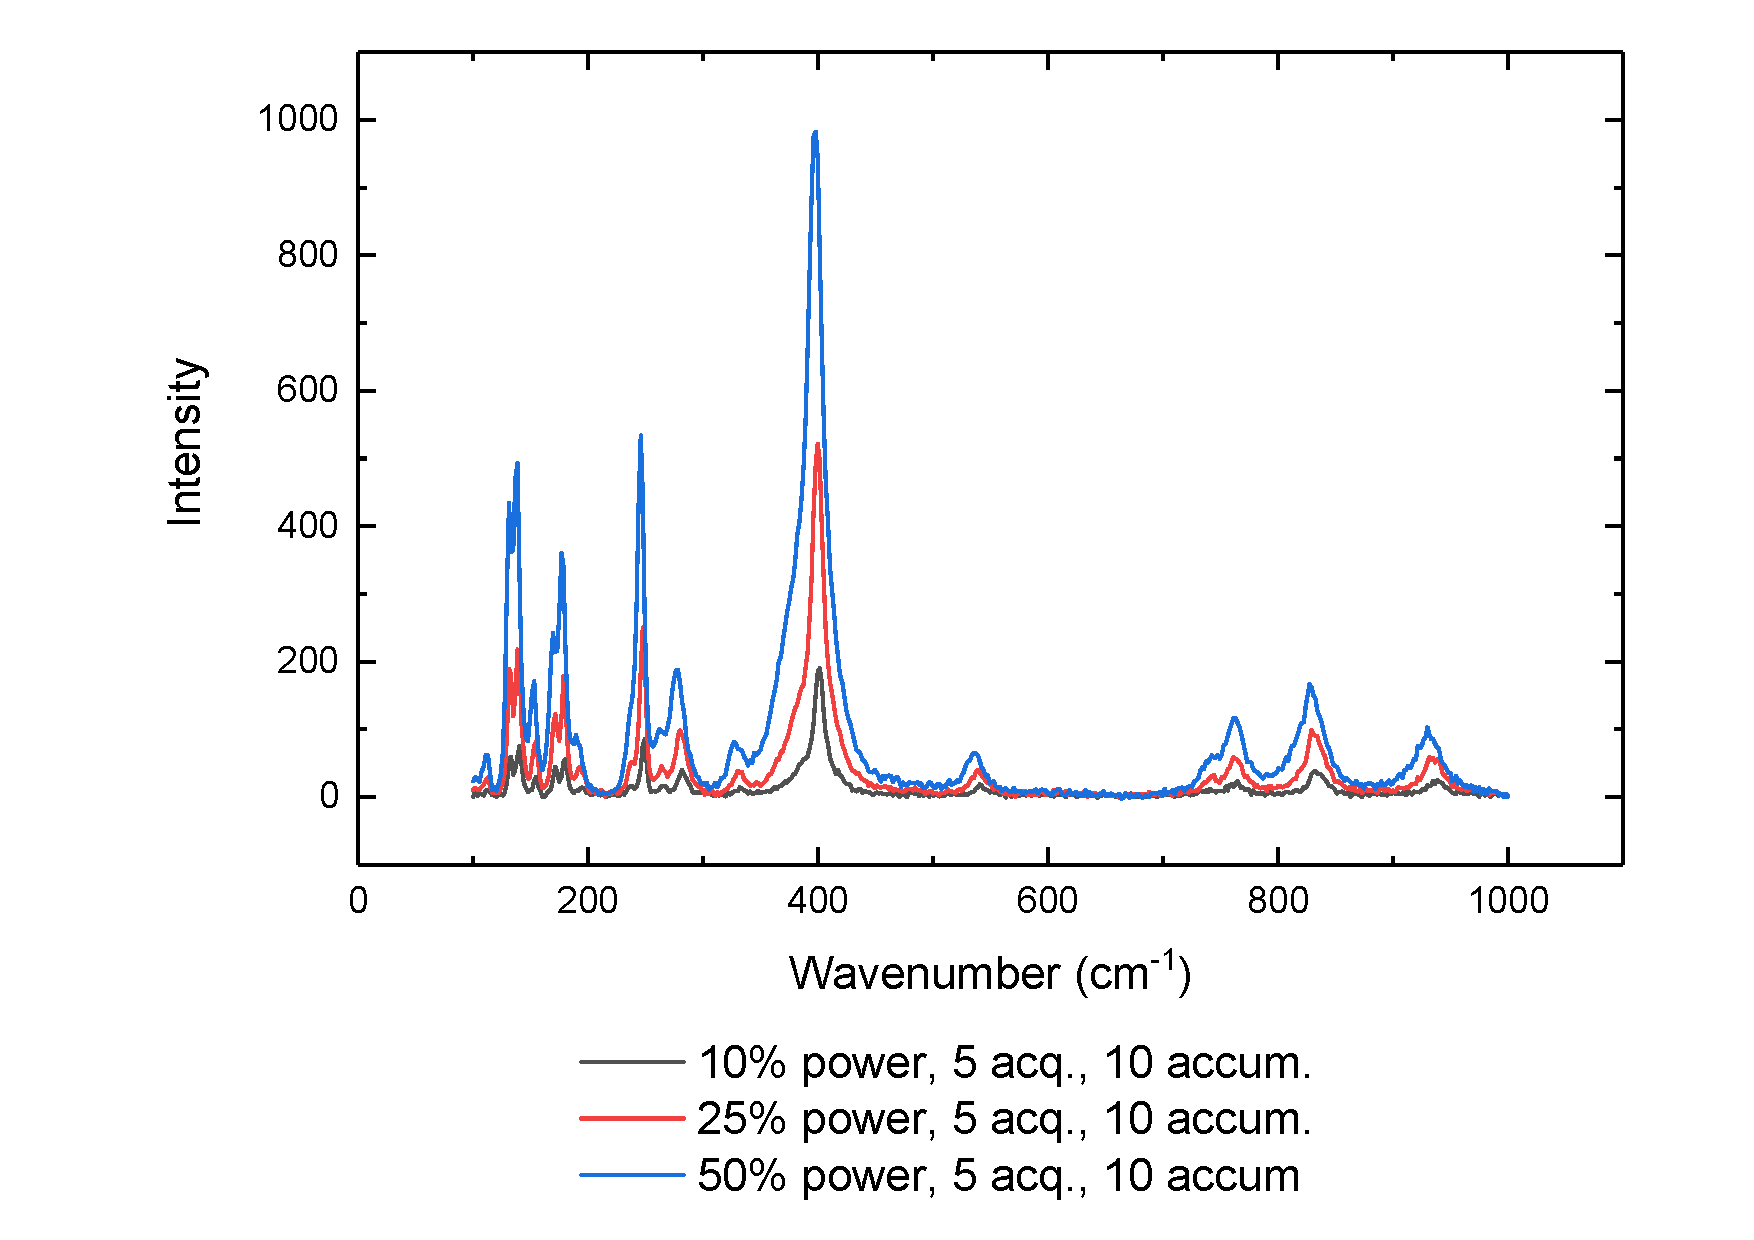
\includegraphics[width=0.75\linewidth]{Az1_laserpower_comp_532}
\caption[Comparison of spectra collected using 532 nm excitation wavelength at 10\%, 25\%, and 50\% power.]{Comparison of spectra collected using 532 nm excitation wavelength at 10\% (black), 25\% (red), and 50\% (blue) power (5 acquisitions, 10 accumulations).}
\label{fig:Az1_laserpower_comp_532}
\end{figure}

Raman spectra were processed using OriginPro 2017 software. All spectra were fit to a spline baseline. 

\section[Analysis of pigment particles by SEM-EDS]{Analysis of pigment particles by SEM-EDS}
\label{section2.3}

Pigment particle morphology and composition were characterized using scanning electron microscopy (SEM) coupled to energy dispersive X-ray spectroscopy (EDS). Micrographs of pigments were collected at several magnifications using a JEOL JSM-5510LV scanning electron microscope using the secondary electron (SE) detector. The sample working distance was 20 mm. The accelerating voltage was 10 keV unless otherwise noted. ED spectra were collected using an Oxford instruments INCA EDX detector and software. Elemental mapping was carried out to detect variation between pigment grains.

Resin embedded cross sections were studied using the same procedure, substituting the SE detector for the backscatter (BSE) detector. Prior to SEM-EDS analysis, cross sections were coated with a 25 nm layer of amorphous carbon and wrapped with copper metal.

\section[Analysis of pigment particles by AFM-IR]{Analysis of pigment particles by AFM-IR}
\label{section2.4}

Resin-embedded powders and cross sections were studied using an Anasys NanoIR2 instrument in contact and tapping modes. Height, deflection, and phase maps were collected in tapping mode using a HQ:NSC15 Al probe (Mikro Masch, 265-410 kHz resonant frequency, 20-80 N/m force constant). Map areas ranged from 80 x 80 $\mu$m to 2 x 2 $\mu$m with resolution of 250 x 250 pixels and scan rate 0.1 Hz. 

Infrared maps and spectra were collected in contact mode using an ATEC-CONTAu-10 gold-coated silicon probe (7-25 kHz resonant frequency, 0.02-0.75 N/m spring constant, Nanosensors). Four quantum cascade lasers (Daylight Solutions, 10.98\% power) spanning a total range of 1125-2298 cm\textsuperscript{-1} were used. Infrared mapping was done at several frequencies discussed in analysis.

%The duty cycle was 3\%. 

\section[Bulk sample analysis by ATR FT-IR]{Bulk sample analysis by attenuated total reflectance infrared spectroscopy}
\label{section2.5}

Attenuated total reflectance (ATR) infrared spectra were collected using a Bruker Vertex 70 FT-IR spectrometer (Goldengate ATR accessory, liquid nitrogen cooled MCT mid-IR detector, OPUS software). A background spectrum was collected before each sample spectrum using the clean ATR crystal (200 scans). Each sample spectrum was collected from solid powder/resin (200 scans, resolution 4 cm\textsuperscript{-1}). Spectra were processed using OriginPro 2017 by fitting a spline baseline to transmission spectra and subtracting. Data was converted from transmittance to absorbance as needed for comparison to AFM-IR spectra.


